%% Copyright (C)  2011 Jefferson Campos, Kleber Souza,
%% Lucas Apolinário, Ruan Castelo.
%% Permission is granted to copy, distribute and/or modify this document
%% under the terms of the GNU Free Documentation License, Version 1.3
%% or any later version published by the Free Software Foundation;
%% with no Invariant Sections, no Front-Cover Texts, and no Back-Cover Texts.
%% A copy of the license is included in the section entitled "GNU
%% Free Documentation License".

\documentclass[a4paper,12pt]{article}
\usepackage[brazilian]{babel}
\usepackage[utf8]{inputenc}
\usepackage[T1]{fontenc}
\usepackage{hyperref}
\usepackage{url}
\usepackage[pdftex]{graphicx}
\newcommand{\HRule}{\rule{\linewidth}{0.5mm}}

\begin{document}

\begin{titlepage}

\begin{center}


\includegraphics[width=0.15\textwidth]{./ufscar.jpg}\\[1cm]    

\textsc{\LARGE UNIVERSIDADE FEDERAL DE SÃO CARLOS}\\[1.5cm]

\textsc{\Large UFSCAR}\\[0.5cm]

\HRule \\[0.4cm]
{ \huge \bfseries Prova de continuídade para $(g \circ f)(x,y)$.}\\[0.4cm]

\HRule \\[1.5cm]


\begin{minipage}{0.4\textwidth}
\begin{flushleft} \large
\emph{Autor:}\\
Jefferson \textsc{Campos}\\
RA 423114\\
\end{flushleft}
\end{minipage}
\begin{minipage}{0.4\textwidth}
\begin{flushright} \large
\emph{Supervisor:} \\
Dra. Silvia Maria Simões de  \textsc{Carvalho}
\end{flushright}
\end{minipage}

\vfill

{\large \today}

\end{center}

\end{titlepage}


\section{Cibernética.}

\begin{itemize}
\item Definição: comunicação e o controle de máquinas, seres vivos e grupos sociais;
\item Distinção entre robótica e cibernética (confusão com termo CYBORG)
\item Estudo da informação:
\begin{itemize}
\item codificação/descodificação;
\item retroação ou realimentação (feedback);
\item aprendizagem (IA - inteligência artificial);
\end{itemize}
\item Não há distinção entre serves vivos e máquinas;
\item Rompimento com causalidade linear - introdução do mecanismo de feedback
\begin{itemize}
\item Regulação: A --> B, B --> A
\item Base para sistemas autonomos e aprendizado
\end{itemize}
\item Aplicações:
\begin{itemize}
\item militar
\begin{itemize}
\item armas biológicas
\end{itemize}
\item economica
\begin{itemize}
\item US, URSS, França...
\end{itemize}
\end{itemize}
\end{itemize}

\section{Teoria de Sistemas.}

\subsection{Histórico.}
\begin{itemize}
\item proposta em 1937 pelo biólogo Ludwig von Bertalanffy;
\item A teoria de sistemas, cujos primeiros enunciados datam de 1925, foi  tendo alcançado o seu auge de divulgação na década de 50; 
\item Em 1956 Ross Ashby introduziu o conceito na ciência cibernética;
\item A pesquisa de Von Bertalanffy foi baseada numa visão diferente do reducionismo científico até então aplicada pela ciência convencional.
\end{itemize}

\subsection{Conceitos.}
\begin{itemize}
\item Entropia - todo sistema sofre deteriorização;
\item Sintropia, negentropia ou entropia negativa - para que o sistema continue existindo, tem que desenvolver forças contrárias à Entropia;
\item Homeostase - capacidade do sistema manter o equilibrio;
\item Homeorrese - toda vez que há uma ação imprópria (desgaste) do sistema, ele tende a se equilibrar.
\item Definição de escopo - Sistemas abertos/fechados;
\item Realimentações (cibernética);
\item O Sistema é um conjunto de partes interagentes e interdependentes que, conjuntamente, formam um todo unitário com determinado objetivo e efetuam determinada função;
\item Sistema pode ser definido como um conjunto de elementos interdependentes que interagem com objetivos comuns formando um todo, e onde cada um dos elementos componentes comporta-se, por sua vez, como um sistema cujo resultado é maior do que o resultado que as unidades poderiam ter se funcionassem independentemente. Qualquer conjunto de partes unidas entre si pode ser considerado um sistema, desde que as relações entre as partes e o comportamento do todo sejam o foco de atenção;
\item Sistema é um conjunto de partes coordenadas, formando um todo complexo ou unitário;
\end{itemize}


\subsection{Interdisciplinaridade.}
\begin{itemize}
\item Em biologia temos nas células um exemplo, pois não importa quão profundo o estudo individual de um neurônio do cérebro humano, este jamais indicará o estado de uma estrutura de pensamento, se for estirpado, ou morrer, também não alterará o funcionamento do cérebro.
\item Uma área emergente da biologia molecular moderna que se utiliza bastante dos conceitos da Teoria de Sistemas é a Biologia Sistêmica - que estuda e projeta as relações dinâmicas entre as moléculas dos organismos vivos.
\item Os mesmos conceitos e princípios que orientam uma organização no ponto de vista sistêmico, estão em todas as disciplinas, físicas, biológicas, tecnológicas, sociológicas, etc. provendo uma base para a sua unificação.
\end{itemize}

\section{Modelos Computacionais.}

\subsection{Linguagem R.}
\begin{itemize}
\item \url{http://www.r-project.org/}
\item Foi criada originalmente por Ross Ihaka e por Robert Gentleman no departamento de Estatística da universidade de Auckland, Nova Zelândia, e foi desenvolvido por um esforço colaborativo de pessoas em vários locais do mundo.
\end{itemize}

\section{Ferramentas.}
\begin{itemize}
\item Fluxograma (exemplo - sites em anexo)
\item UML (exemplo .png em anexo)
\item Modelos Matemáticos:
\begin{itemize}
\item Função (função exponencial - crescimento de uma bactéria - exemplo sites em anexo) 
\end{itemize}
\end{itemize}

\subsection{Exemplos.}
\subsubsection{UML.}
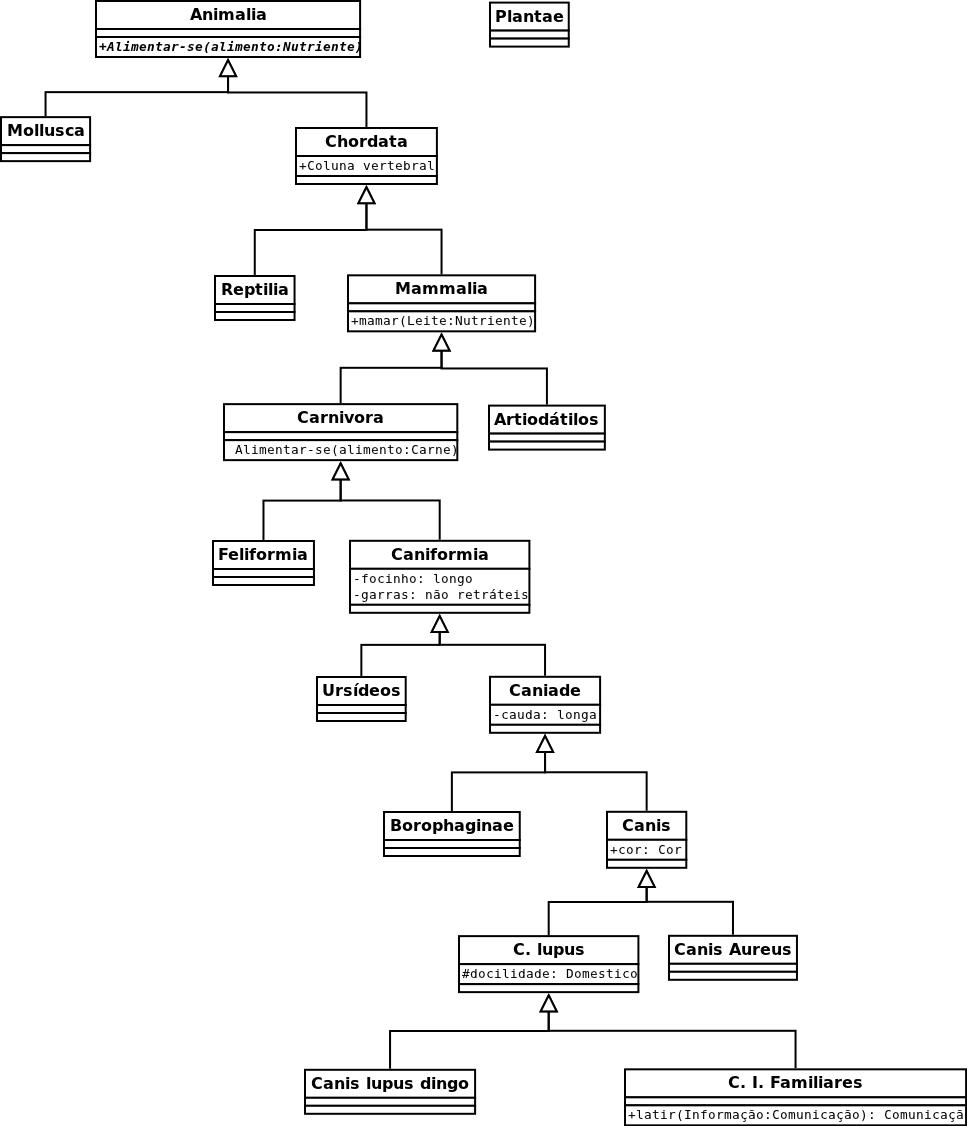
\includegraphics[width=1.15\textwidth]{./seminar_ecology.png}\\[1cm]

\section{Licença.}

Copyright (C)  2011 Jefferson Campos, Kleber Souza,\\
Lucas Apolinário, Ruan Castelo.\\
Permission is granted to copy, distribute and/or modify this document\\
under the terms of the GNU Free Documentation License, Version 1.3\\
or any later version published by the Free Software Foundation;\\
with no Invariant Sections, no Front-Cover Texts, and no Back-Cover Texts.\\
A copy of the license is included in the section entitled "GNU\\
Free Documentation License".

\nocite{MUNARI:2006}
\nocite{website:simulacao}
\nocite{website:cibernetica}
\nocite{website:cibernetica_GEROVITCH}
\nocite{website:cibernetica_MEDINA}
\nocite{website:cibernetica_WIENER}
\nocite{website:teoria_sistemas}
\nocite{texbook:teoria_sistema_KLIR}
\nocite{texbook:teoria_sistema_CHIAVENATO}
\nocite{texbook:teoria_sistema_BERTALANFFY}
\nocite{texbook:teoria_sistema_CAPRA}
\nocite{website:r_project}
\bibliographystyle{ieeetr}
\bibliography{seminar_ecology}

\end{document}

